% Settings for the default beamer theme
\documentclass[english, aspectratio=169]{beamer}
\usepackage{babel}
\usepackage{tabularx}
\usepackage[T1]{fontenc}
\usepackage[utf8]{inputenc}
\usepackage[ruled,vlined]{algorithm2e}
\setcounter{secnumdepth}{3}
\setcounter{tocdepth}{3}

\makeatletter

\newcommand\makebeamertitle{\frame{\maketitle}}

% (ERT) argument for the TOC
\AtBeginDocument{%
  \let\origtableofcontents=\tableofcontents
  \def\tableofcontents{\@ifnextchar[{\origtableofcontents}{\gobbletableofcontents}}
  \def\gobbletableofcontents#1{\origtableofcontents}
}

% Theme settings
\usetheme{Frankfurt}
\usecolortheme{default}
\usefonttheme[onlymath]{serif}

% Template settings
\setbeamertemplate{navigation symbols}{}
\setbeamertemplate{blocks}[rounded][shadow=false]
\setbeamertemplate{title page}[default][colsep=-4bp, rounded=true, shadow=false]
\makeatother

\begin{document}

% Title page
\section{Bevezetés}
\title[]{Üzleti Intelligencia}
\subtitle{3. Előadás: Markov döntési folyamatok megoldása}
\author[Kuknyó Dániel]{Kuknyó Dániel\\Budapesti Gazdasági Egyetem}
\date{2023/24\\1.félév}
\makebeamertitle

% Table of contents slide
\begin{frame}
\tableofcontents{}
\end{frame}

% Table of contents of the current section
\begin{frame}
\tableofcontents[currentsection]
\end{frame}

\begin{frame}{Az RL modellje}
\begin{columns}
\begin{column}{.5\textwidth}
\only<1>{\begin{block}{Markov döntési folyamat}
\[
\left(S,A,P,R,s_{0},\gamma\right)
\]
\begin{itemize}
	\item $S$: állapotok halmaza
	\item $A$: cselekvések halmaza
	\item $P:\; S \times A \times S \rightarrow [0,1]$: állapotátmeneti valószínűségek
	\item $R:\; S \times A \rightarrow \mathbb{R}$: azonnali jutalmak halmaza
	\item $s_{0}$: kezdőállapot
	\item $\gamma$: diszkont faktor
\end{itemize}
\end{block}}
\only<2>{Az MDP folyamata:\\
\begin{enumerate}
	\item Az ügynök $s_{0}$ állapotból indul
	\item Az ügynök $\pi$ politika szerint cselekszik: $a_{t}\sim\pi(s_{t})$
	\item A környezet reagál a cselekvésre, és visszaadja az ügynöknek $r_{t+1}$ jutalmat és $s_{t+1}$ következő állapotot
	\item Ez ismétlődik amíg a kilépési kritérium be nem teljesül
\end{enumerate}
Cél: Az optimális politika megtalálása. A politika optimális, ha a hozamának várható értéke maximális:
\[
E_{\pi}\left(r_{1} + \gamma r_{2} + \gamma^{2}r_{3} + ...\right) \rightarrow max
\]}
\end{column}
\begin{column}{.5\textwidth}
\begin{center}
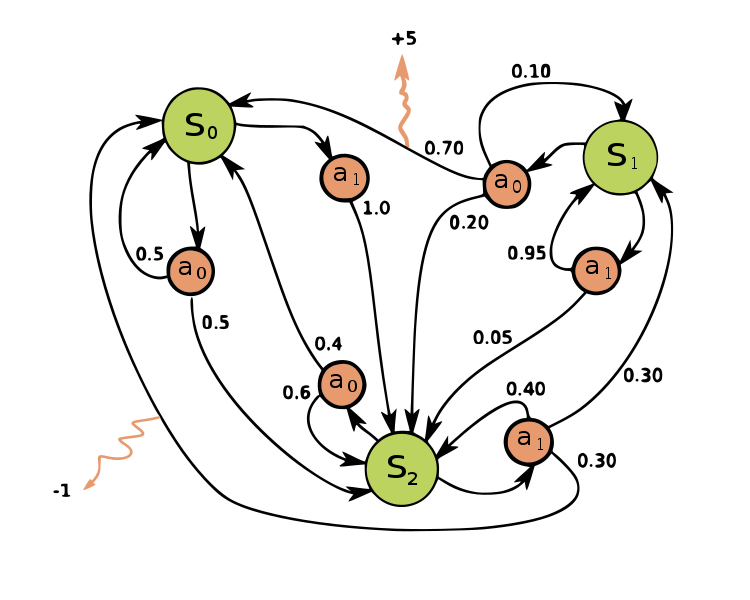
\includegraphics[width=7cm, height=7cm, keepaspectratio]{images/solving_1.png}
\end{center}
\end{column}
\end{columns}
\end{frame}

\begin{frame}{A mohó ügynök}
\begin{columns}[T]
\begin{column}{.5\textwidth}
A legegyszerűbb cselekvés kiválasztási szabály, ha az ügynök mindig azt a cselekvést választja, ami számára a lehető legnagyobb várható hozammal rendelkezik.
\begin{center}
\begin{block}{Mohó cselekvés választás}
Mohó politika mindig azt a cselekvést fogja választani, amelyik - egy lépéses távlatban - a lehető legnagyobb várható jutalommal fog járni az ügynök számára $v_{\pi}$ szerint.
\[
A_{t}=\underset{a}{argmax}\:Q_{t}(a)
\]
\end{block}
\end{center}
\end{column}
\begin{column}{.5\textwidth}
\begin{itemize}
	\item Mi lenne a mohó politika ebben az estben?
	\item Mindig ez a legjobb megoldás?
	\item A legjobb megoldás mindig mohó?
\end{itemize}
\begin{center}
\only<1>{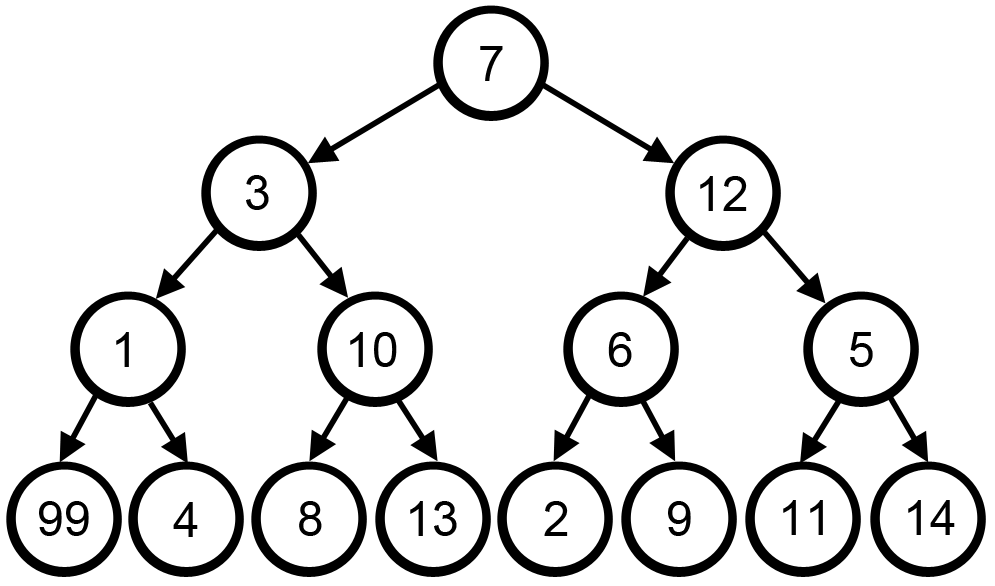
\includegraphics[width=7cm, height=7cm, keepaspectratio]{images/solving_2.png}}
\only<2>{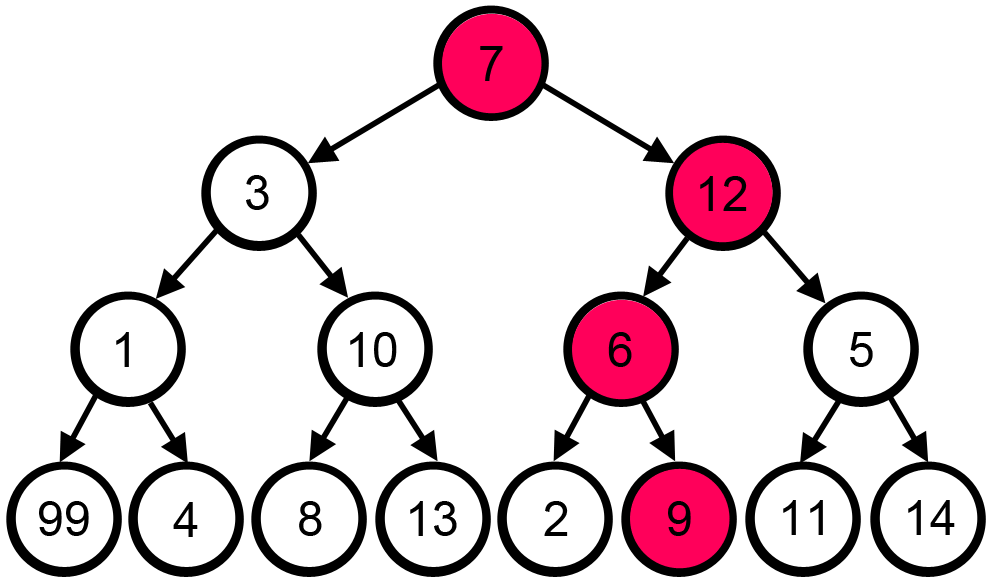
\includegraphics[width=7cm, height=7cm, keepaspectratio]{images/solving_3.png}}
\end{center}
\end{column}
\end{columns}
\end{frame}

\begin{frame}{Az $\varepsilon$-mohó stratégia}
\begin{columns}
\begin{column}{.5\textwidth}
Egy másik lehetőség, ha adott valószínűséggel az ügynök véletlen cselekvést hajt végre remélve, hogy ezzel elér egy olyan állapotba amelyhez nagy jutalom tartozik. A véletlen cselekvés a \textbf{felfedezés}, és végrehajtásának valószínűsége $\epsilon$.
\begin{center}
\begin{block}{$\varepsilon$-mohó cselekvés választás}
\[
A_{t}\leftarrow\begin{cases}
_{a\sim A}^{\underset{a}{argmax}Q(a)} & _{P=\varepsilon}^{P=1-\varepsilon}\end{cases}
\]
\end{block}
\end{center}
\end{column}
\begin{column}{.5\textwidth}
Az ügynök tehát $\varepsilon$ valószínűséggel véletlen cselekvést választ az ismeretlen, de nagyobb jutalom reményében. Ez a \textbf{felfedezés} művelete.\\
$\varepsilon$ valószínűséggel pedig a már ismert és a legnagyobb várható jutalommal járó cselekvést hajtja végre. Ez a \textbf{kizsákmányolás} művelete.
\begin{center}
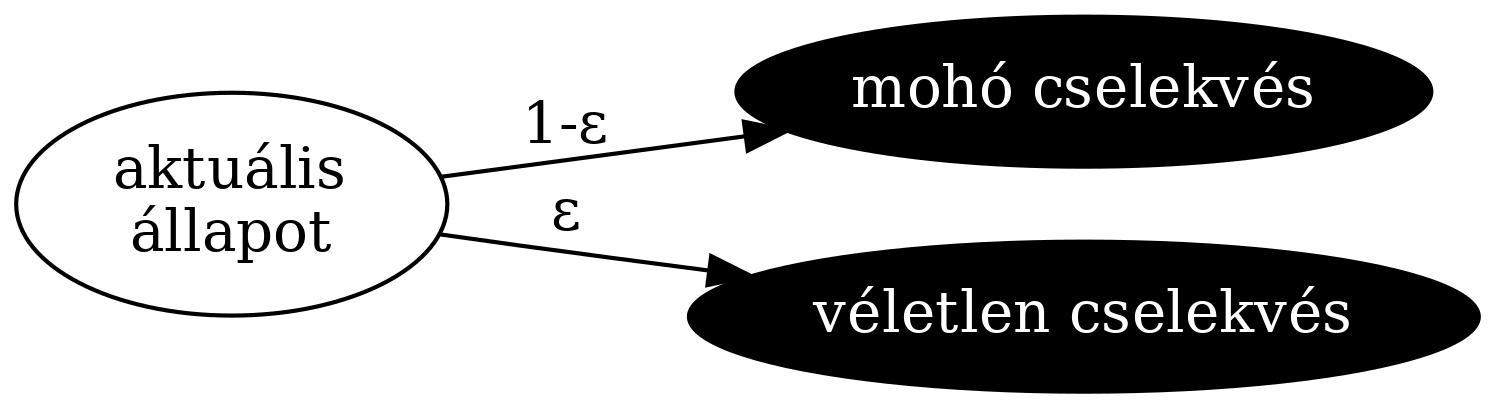
\includegraphics[width=7cm, height=6cm, keepaspectratio]{graphs/solving_1.png}
\end{center}
\end{column}
\end{columns}
\end{frame}

\begin{frame}{Példák}
A következő valós példák alkalmasak a felfedezés/kizsákmányolás dilemma bemutatására:
\begin{itemize}
	\item Étterem választás:
	\begin{itemize}
		\item \textbf{Kizsákmányolás}: elmész a kedvenc éttermedbe.
		\item \textbf{Felfedezés}: elmész egy új étterembe, hátha találsz egy jobbat mint a kedvenced.
	\end{itemize}
	\item Online hirdetés:
	\begin{itemize}
		\item \textbf{Kizsákmányolás}: a legjobb reklám megmutatása a felhasználónak.
		\item \textbf{Felfedezés}: egy új reklám megmutatása a felhasználónak, hátha tetszik neki.
	\end{itemize}
	\item Olajfúrás:
	\begin{itemize}
		\item \textbf{Kizsákmányolás}: Egy meglévő helyen fúrás az olajért.
		\item \textbf{Felfedezés}: Egy új helyen fúrás.
	\end{itemize}
	\item Klinikai kezelés:
	\begin{itemize}
		\item \textbf{Kizsákmányolás}: A bevált kezelés alkalmazása.
		\item \textbf{Felfedezés}: Új kezelés kipróbálása.
	\end{itemize}
\end{itemize}
\end{frame}

\section{A rabló probléma}

\begin{frame}
\tableofcontents[currentsection]
\end{frame}

\begin{frame}{A rabló probléma}
\begin{columns}
\begin{column}{.5\textwidth}
\only<1>{A $k$-karú rabló problémája egy elméleti megerősítéses tanulás probléma. A játékos egy rablógépen játszik, amelynek $k$ karja van. \\
Minden karhúzás után egy állandó eloszlásból választott jutalmat kap az ügynök. Az ügynök célja, hogy olyan politikát válasszon, ami az elvárt hozamot maximalizálja $1000$ cselekvés vagy \emph{időlépés} után.}
\only<2>{Az ügynöknek számon kell tartania, mennyi a jutalom várható értéke, ha adott egy $a$ cselekvés. Ez a $Q(s,a)$ állapot-cselekvés minőség függvény. A rabló problémában csak egy állapot van, ezért elég csak a cselekvésekhez tartozóan számon tartani:
\[
q_{*}(a)=E\left[r_{t}|A_{t}=a\right]
\]
A jutalom várható értéke: 
\[
Q_{n}=\frac{r_{1}+r_{2}+...+r_{n-1}}{n-1}
\]
}
\end{column}
\begin{column}{.5\textwidth}
\begin{center}
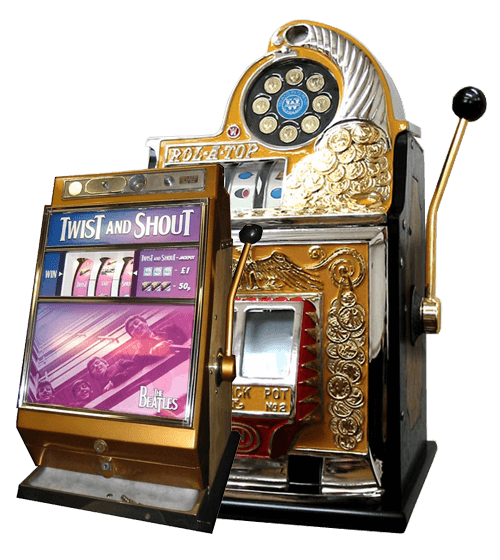
\includegraphics[width=7cm, height=7cm, keepaspectratio]{images/solving_5.png}
\end{center}
\end{column}
\end{columns}
\end{frame}

\begin{frame}{Algoritmus a rabló megoldására}
\begin{algorithm}[H]
\caption{Egyszerű rabló algoritmus}
\SetAlgoLined
	$Q(a)\leftarrow0\;for\;a=1\rightarrow k$\tcc*[r]{Cselekvés minőségének függvénye}
	$N(a)\leftarrow	0\;for\;a=1\rightarrow k$\tcc*[r]{Kar meghúzásainak a száma}
	\For{$t=1 \rightarrow max_{t}$}{
		$p=random(0,1)$\tcc*[t]{Véletlen szám $0$ és $1$ között}
		\eIf{$p>\varepsilon$}{
			$a \leftarrow \underset{a}{argmax}Q(a)$\tcc*[r]{Legnagyobb ismert jutalom cselekvése}
		}{
			$a \leftarrow a \sim A $\tcc*[r]{Véletlen cselekvés}
		}
		$r\leftarrow env(a)$\tcc*[t]{Cselekvés végrehajtása a környezetben}
		$N(a) \leftarrow N(a)+1$\tcc*[t]{Cselekvés számlálójának növelése}
		$Q(a) \leftarrow Q(a) + \frac{1}{N(a)}\left[r-Q(a)\right]$\tcc*[t]{$Q$-érték frissítése}
	}
\end{algorithm}
\end{frame}

\begin{frame}{Egy példa rabló}
\begin{columns}
\begin{column}{.5\textwidth}
Hogy meg lehessen mérni a mohó és $\varepsilon$-mohó stratégiák teljesítményét, szükség van egy teszt rablóra. A példában szereplő egy $10$-karú rabló. Minden karhoz tartozóan a jutalmak eloszlása Gauss-i eloszlást követ $1$ varianciával, viszont nem $0$ átlaggal. \par\smallskip
Valamelyik karok nagyobb valószínűséggel járnak magas jutalommal mint a többi. Az ügynök feladata megtalálni melyik kartól remélhet nagyobb jutalmat. Ehhez szükség van arra, hogy végig próbálja őket.
\end{column}
\begin{column}{.5\textwidth}
\begin{center}
A jutalmak eloszlása
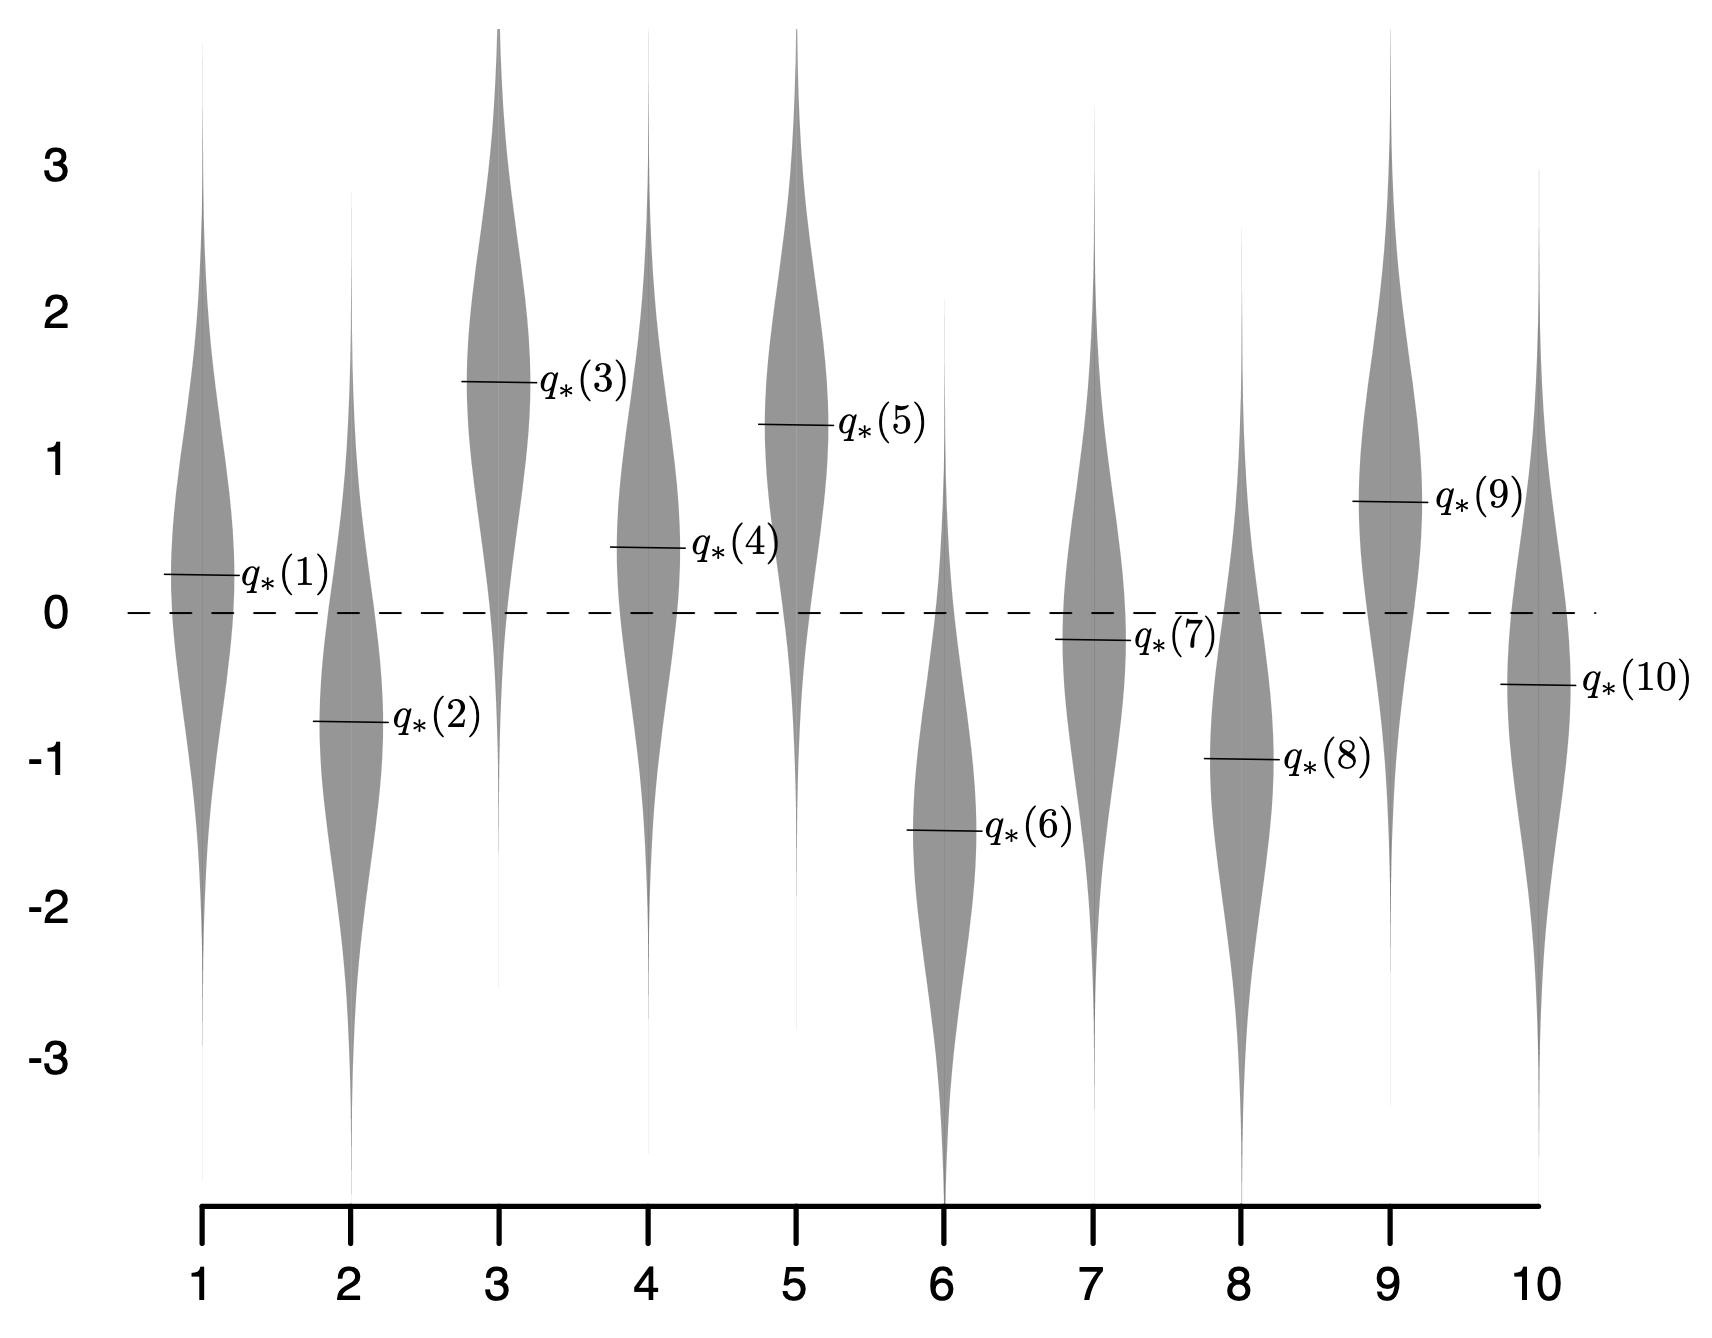
\includegraphics[width=7cm, height=6cm, keepaspectratio]{images/solving_6.png}
\begin{scriptsize}
Cselekvés
\end{scriptsize}
\end{center}
\end{column}
\end{columns}
\end{frame}

\begin{frame}{A futás teljesítménye}
\begin{columns}
\begin{column}{.5\textwidth}
Az algoritmus $1000$ időlépésen keresztül futott $\varepsilon=0,\varepsilon=0.01,\varepsilon=0.001$ hiperparaméterekkel. Minél nagyobb a $\varepsilon$ érték, annál nagyobb a felfedezés valószínűsége. \par\smallskip 
Mindegyik módszer megbecsülte az állapot-cselekvés minőség függvényt a rabló minden karára a mozgóátlagolás technikájával. A diagramon a várható jutalom mértékét mutatja az időlépések függvényében. 
\par\smallskip
A mohó stratégia kezdetben gyorsabban javult mint a többi, de kisebb értékre konvergált a futásidő végére.
\end{column}
\begin{column}{.5\textwidth}
\begin{center}
Átlagos jutalom
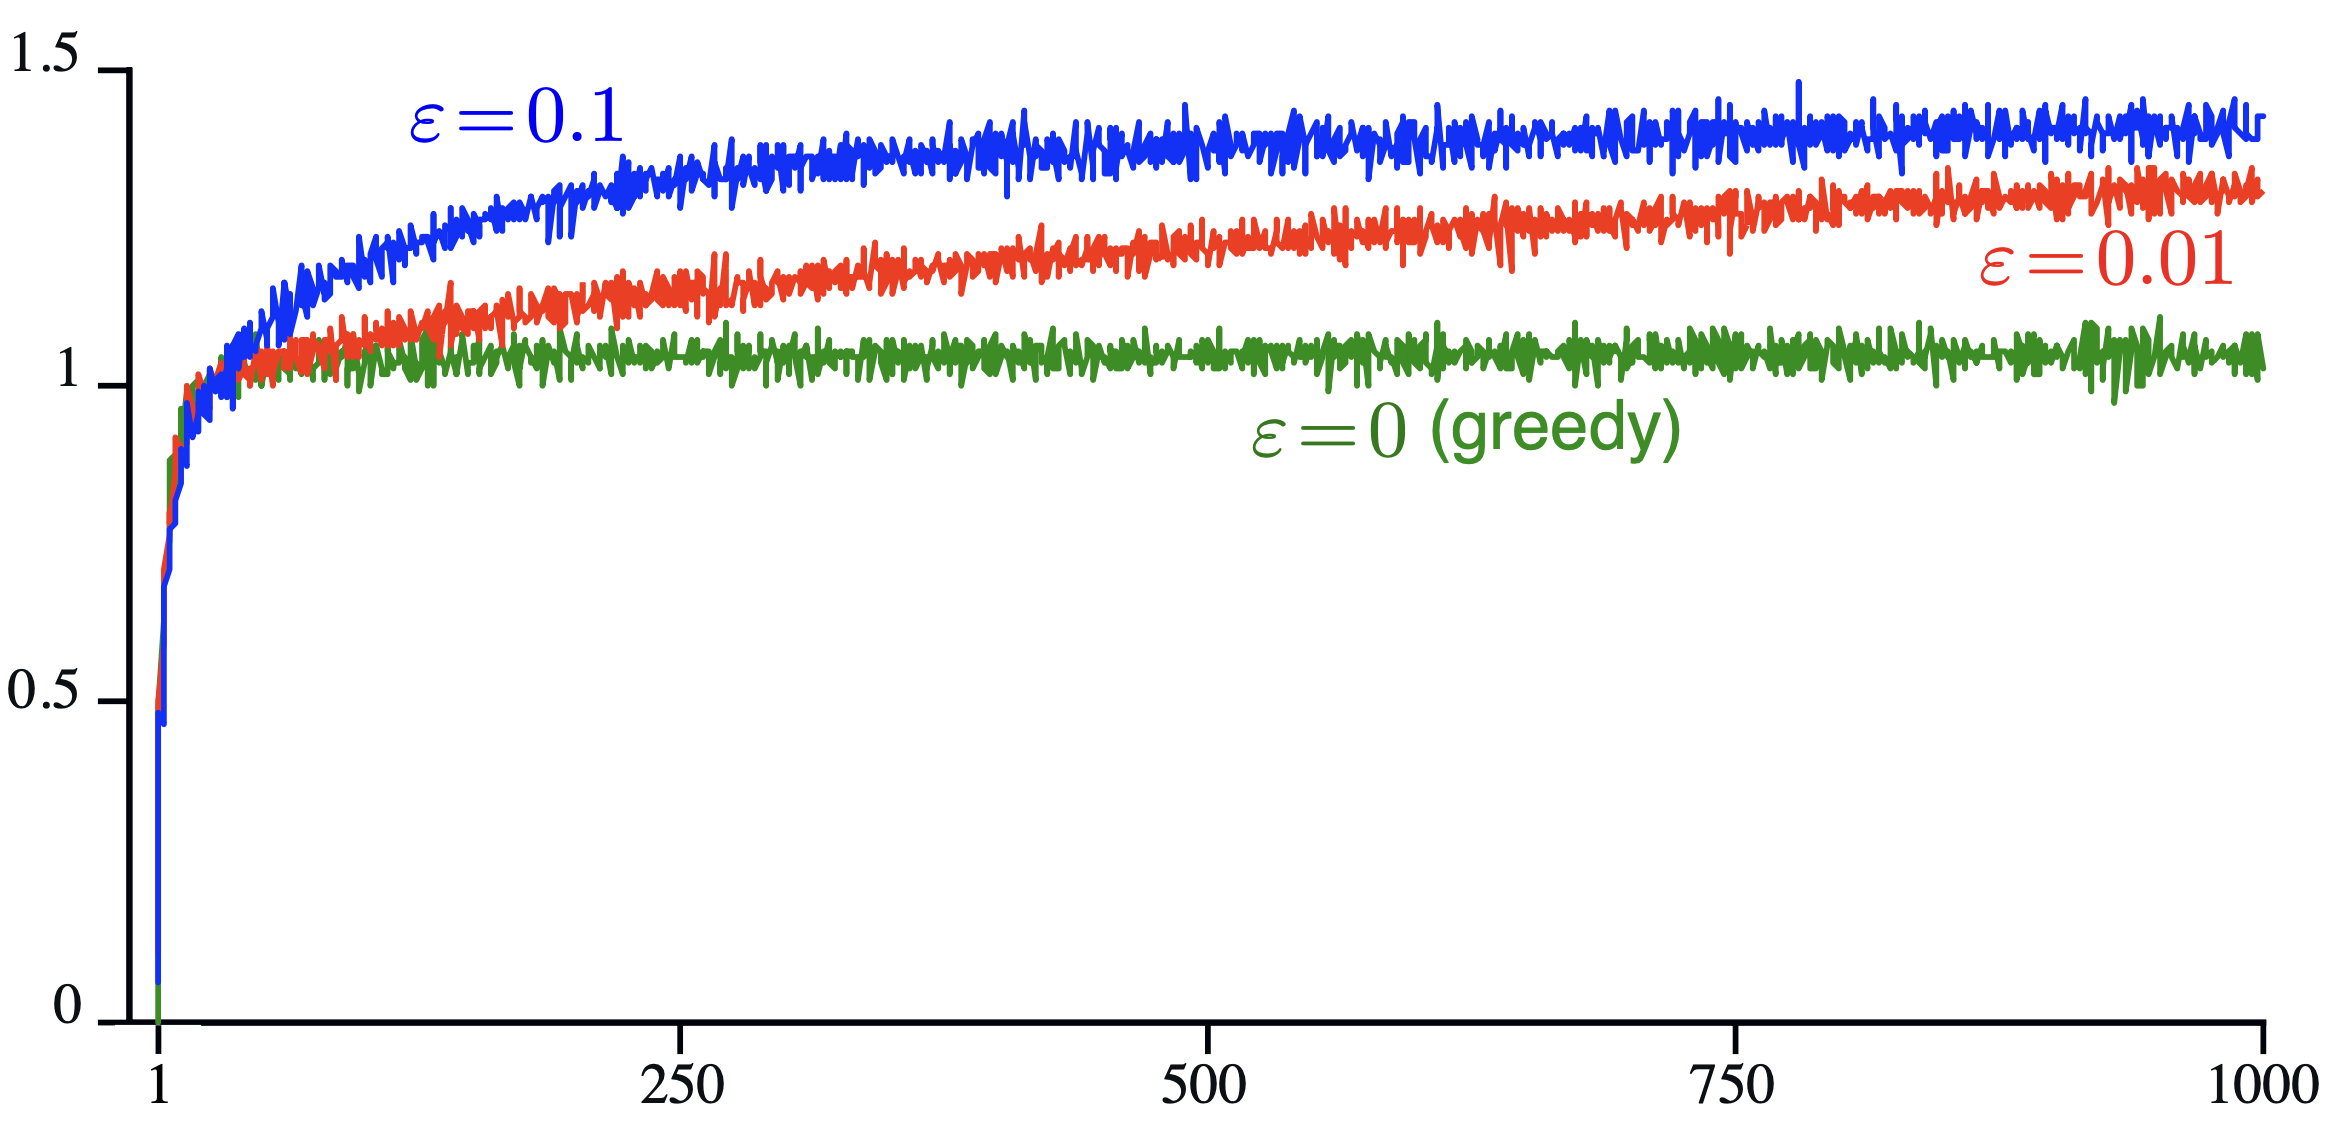
\includegraphics[width=7cm, keepaspectratio]{images/solving_7.png}
\begin{scriptsize}
Időlépés
\end{scriptsize}
\end{center}
\end{column}
\end{columns}
\end{frame}

\begin{frame}{A futás teljesítménye}
\begin{columns}
\begin{column}{.5\textwidth}
Az ábra azt mutatja, hogy a mohó módszer csak a feladatok mintegy $30\%$-ában találta meg az optimális műveletet. Az $\varepsilon$-mohó módszerek végül jobban teljesítettek, mert folytatták a felfedezést és javították az esélyüket az optimális művelet felismerésére. \par\smallskip
Az $\varepsilon=0.1$ módszer többet fedezett fel, és általában korábban megtalálta az optimális műveletet, de soha nem választotta ki azt több mint $91\%$-ban. \par\smallskip
Az $\varepsilon=0.01$ módszer lassabban javult, de végül mindkét teljesítménymérőn jobban teljesített.
\end{column}
\begin{column}{.5\textwidth}
\begin{center}
Optimális cselekvés aránya
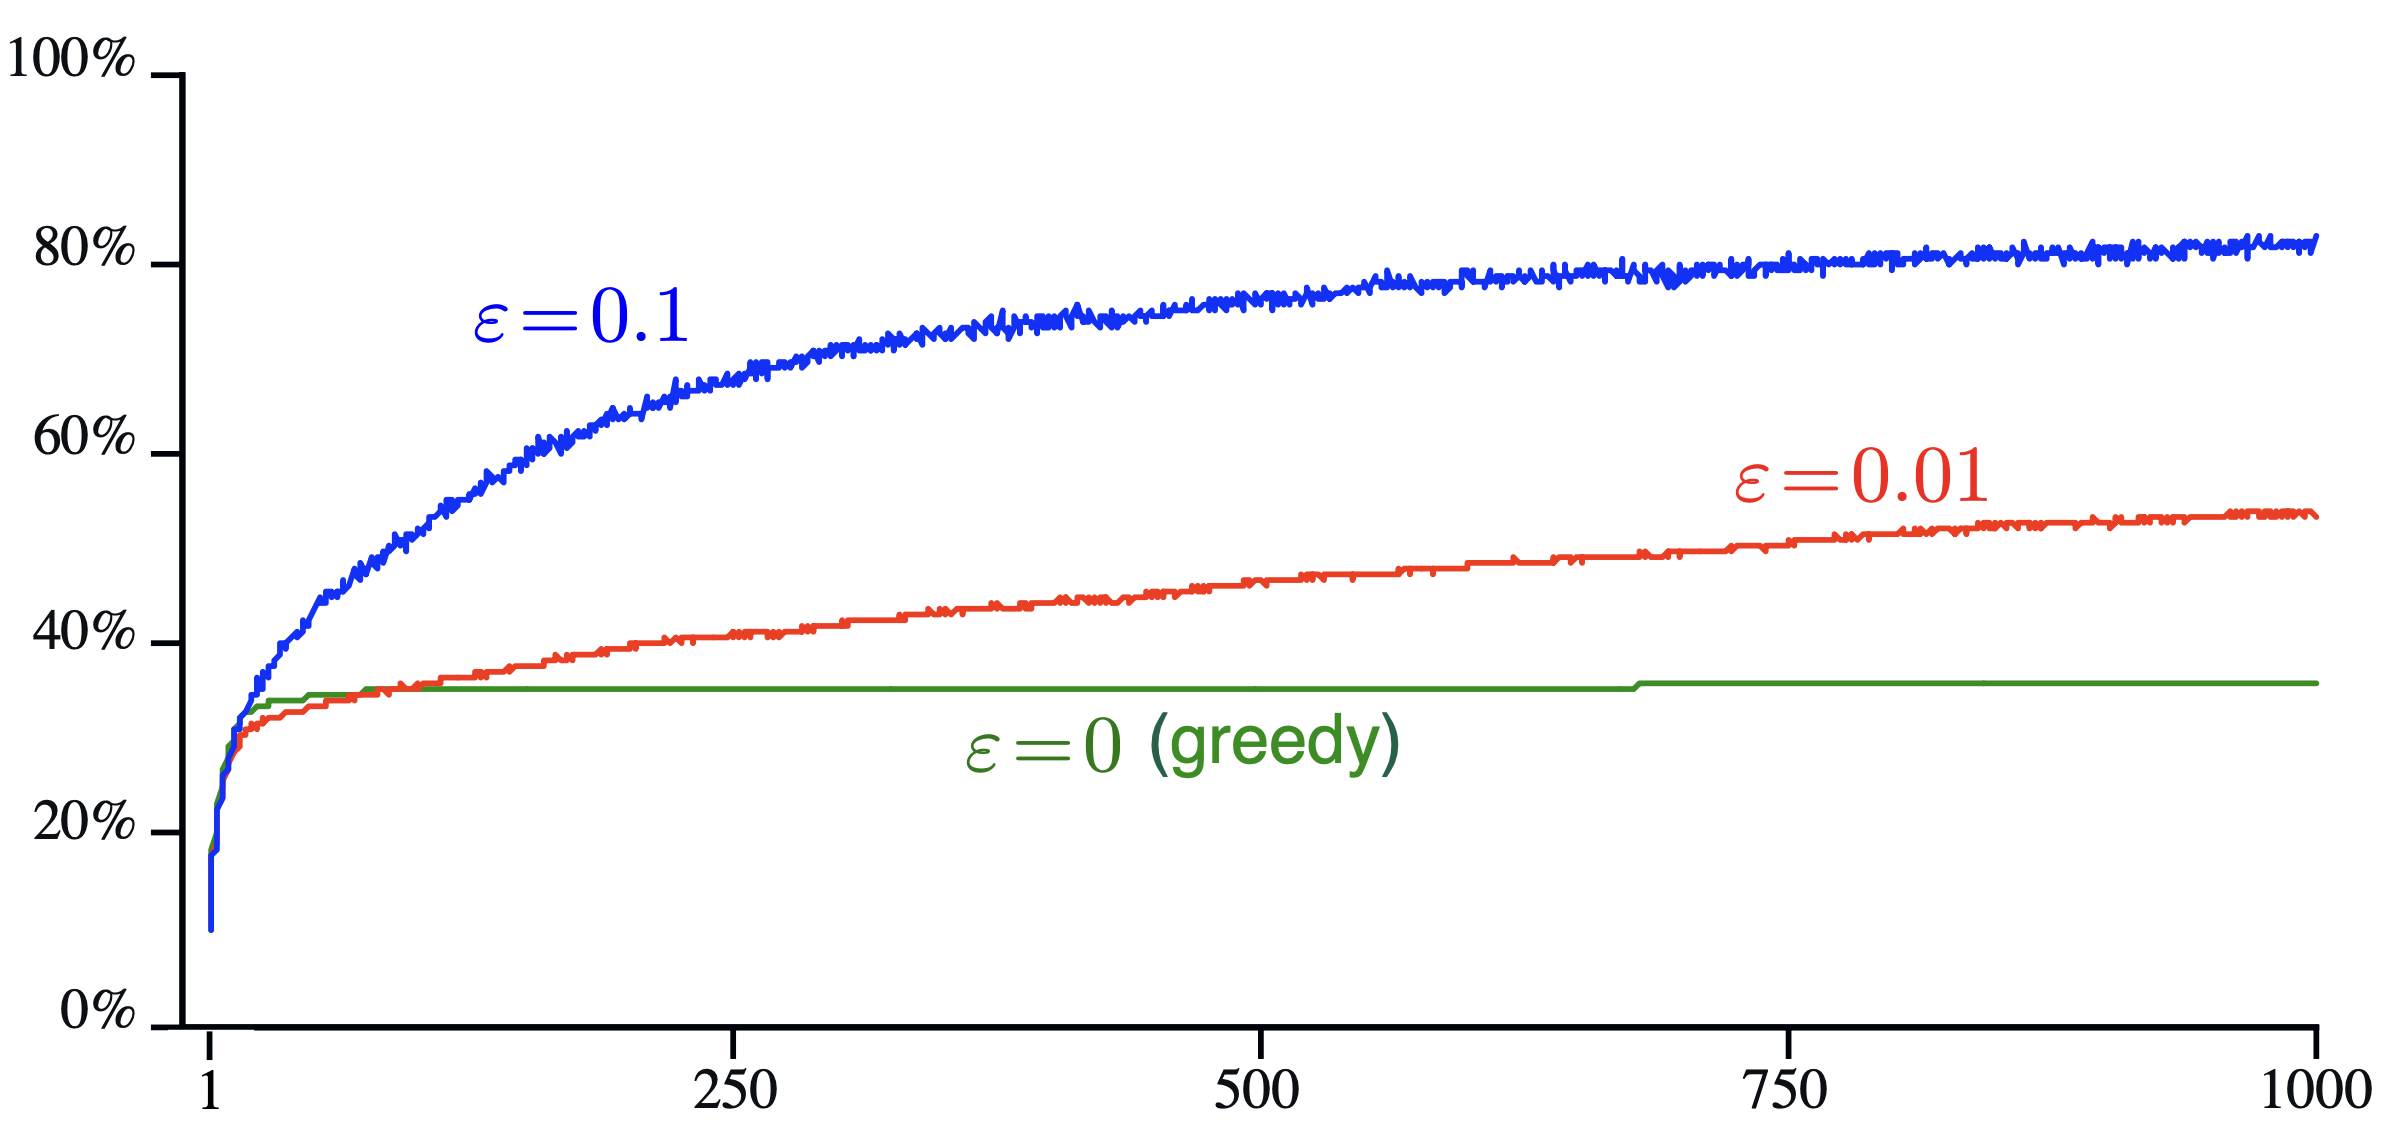
\includegraphics[width=7cm, keepaspectratio]{images/solving_8.png}
\begin{scriptsize}
Időlépés
\end{scriptsize}
\end{center}
\end{column}
\end{columns}
\end{frame}

\section{Dinamikus programozás}

\begin{frame}
\tableofcontents[currentsection]
\end{frame}

\begin{frame}{Dinamikus programozás alapjai}
\begin{columns}
\begin{column}{.5\textwidth}

\only<1>{A dinamikus programozás egy gyűjtőfogalom olyan algoritmusokra amelyekkel kiszámolható az optimális politika \emph{ha adott egy tökéletes környezeti modell egy Markov döntési folyamatként}.\par\smallskip
A klasszikus dinamikus programozási algoritmusok ritkák a megerősítéses tanulásban mert egy tökéletes környezeti modellt feltételeznek és mert rendkívül erőforrásigényesek.}
\only<2>{\begin{center}
\begin{block}{Dinamikus programozás}
A DP algoritmusok a komplex problémákat alproblémákra bontják, majd a végső megoldást az alproblémák megoldásaiból állítják elő. Ehhez két tulajdonságnak kell érvényesnek lennie:
\begin{itemize}
	\item \textbf{Optimális alstruktúra}: Az almegoldásoknak felhasználhatóknak kell lenniük a probléma megoldására.
	\item \textbf{Átfedésben lévő alproblémák}: Bizonyos alproblémák megoldásait többször is fel lehet használni hasonló feladatok elvégzéséhez.
\end{itemize}
\end{block}
\end{center}}
\end{column}
\begin{column}{.5\textwidth}
\begin{center}
\includegraphics[width=7cm, keepaspectratio]{images/%add later}
\end{center}
\end{column}
\end{columns}
\end{frame}

\end{document}












